\documentclass[swedish]{kththesis}

\usepackage{csquotes} % Recommended by biblatex
\usepackage[backend=bibtex, citestyle=ieee, bibstyle=ieee]{biblatex}
\addbibresource{Kandidatexamensarbete.bib} % The file containing our references, in BibTeX format

\usepackage{nameref}
\usepackage{minted}
\usepackage{listings}
\usepackage{caption}
\usepackage{subcaption}
\usepackage{csquotes}
\usepackage{tikz}

\usemintedstyle{bw}
\usetikzlibrary{shapes.geometric, arrows, positioning}

\tikzstyle{defaultnode} = [
	rectangle,
	minimum width=3cm,
	minimum height=1cm,
	text centered,
	draw=black,
]

\tikzstyle{startstop} = [
	rectangle,
	rounded corners,
	minimum width=3cm,
	minimum height=1cm,
	text centered,
	draw=black,
	fill=red!30
]
\tikzstyle{io} = [
	trapezium,
	trapezium left angle=70,
	trapezium right angle=110,
	minimum width=3cm,
	minimum height=1cm,
	text centered,
	draw=black,
	fill=blue!30
]
\tikzstyle{process} = [
	rectangle,
	minimum width=3cm,
	minimum height=1cm,
	text centered,
	draw=black,
	text width=3cm,
	fill=orange!30
]
\tikzstyle{decision} = [
	diamond,
	minimum width=3cm,
	minimum height=1cm,
	text centered,
	draw=black,
	fill=green!30
]
\tikzstyle{arrow} = [thick,->,>=stealth]

\begin{document}

\title{Detta är den svenska titeln}
\alttitle{This is the English translation of the title}
\author{Julius Recep Colliander Celik}
\email{jcelik@kth.se}
\supervisor{Patric Dahlqvist}
\examiner{Anders Västberg}
\principal{LS Elektronik AB}
\programme{Civilingenjör Informationsteknik}
\school{Skolan för elektroteknik och datavetenskap}
\date{\today}

% Frontmatter includes the titlepage, abstracts and table-of-contents
\frontmatter

\titlepage

\begin{abstract}
  Svensk sammanfattning.

\end{abstract}


\begin{otherlanguage}{english}
  \begin{abstract}
    English abstract.

  \end{abstract}
\end{otherlanguage}


\tableofcontents


% Mainmatter is where the actual contents of the thesis goes
\mainmatter

\chapter{Introduktion}
Vad jag känner till är detta det första publikt dokumenterade försöket av att generera ett användargränssnitt från JSON Schema, som är implementerat i något annat än HTML, CSS eller JavaScript. Detta är relevant då JSON Scheman utvecklats med hänsyn till JSON och JavaScript, samtidigt som många andra språk och miljöer skulle kunna dra nytta av funktionaliteten som JSON Schema kan erbjuda. Det är viktigt att JSON Schema fungerar bra med andra språk än JavaScript för att det ska vara ett bra och användbart verktyg.

Examensarbetet handlade om att undersöka möjligheten att skapa en modell för att beskriva och annotera redigerbar data, och sedan automatiskt generera ett användargränssnitt. Det här kapitlet introducerar hela arbetet. Kapitel \ref{sec:intro:bakgrund} ger en bakgrund till arbetet, vilket innefattar både en enkel teoretisk bakgrund, samt en bakgrund till företaget arbetet utfördes hos, samt systemet som arbetet utvecklades mot. Kapitel \ref{sec:intro:problemområde} diskuterar systemet arbetet utvecklades mot i större detalj. Kapitel \ref{sec:intro:problem} presenterar problemet med en frågeställning. Kapitel \ref{sec:intro:hypotes} föreslår en hypotes som arbetet grundar sig på. Kapitel \ref{sec:intro:syfte} och \ref{sec:intro:mål} diskuterar syftet och målet med arbetet. Riskerna diskuteras i Kapitel \ref{sec:intro:risker}. Kapitel \ref{sec:intro:metodval} presenterar metodvalet. Kapitel \ref{sec:intro:avgränsningar} beskriver arbetets omfattning. Resten av rapportens disposition presenteras i kapitel \ref{sec:intro:disposition}.

\section{Bakgrund}
\label{sec:intro:bakgrund}
Det här kapitlet beskriver bakgrunden till varför och i vilka ämnesområden arbetet utfördes, samt för att ge en förståelse för resten av Introduktionen. Kapitel \ref{sec:intro:json} beskriver JSON och JSON Schema vilket är en stor del av teknikerna som arbetet undersökte. Kapitel \ref{sec:intro:mimer} beskriver företaget arbetet utfördes hos, samt systemet som arbetet utvecklades mot.

\subsection{JSON och JSON Schema}
\label{sec:intro:json}
JavaScript Object Notation \textit{(JSON)} är ett textbaserat dataformat för att utbyta data mellan webbtjänster. Till skillnad mot andra alternativ, som exempelvis XML, är det både läsbart för människor och datorer, samtidigt som det är väldigt kompakt, vilket är en anledning till att det är ett av de mest populäraste dataformaten för datautbyte mellan webbtjänster. \cite{Pezoa2016} JSON utvecklades med inspiration till språket ECMAScript \textit{(JavaScript)} men samtidigt programmeringsspråksoberoende, vilket lett till att implementationer för att generera och parsa JSON finns tillgängliga i många olika programmeringsspråk \cite{ECMA2013}. ECMAScript är ett språk som stöds av alla moderna webbläsare, och har därför blivit en kärnteknik för webben.

Trots att JSON är det populäraste dataformatet för datautbyte mellan webbtjänster saknas det ett väletablerat standardiserat ramverk för metadata-definition \cite{Pezoa2016}. En väldigt lovande formell standard är JSON Schema, vilket är ett ramverk som fortfarande utvecklas av Internet Engineering Task Force \textit{(IETF)}. JSON Schema är ett ramverk för att beskriva och annotera JSON-data \cite{A.Wright}. Kapitel \ref{sec:teori} beskriver JSON och JSON Schema i mer detalj.

\subsection{Mimer SoftRadio}
\label{sec:intro:mimer}
Arbetet utfördes hos LS Elektronik AB \textit{(LSE)}, som är ett tekniskt företag, som utvecklar och tillverkar elektroniska produkter \cite{Ehne}. LSE erbjuder bland annat ett radiosystem som heter Mimer SoftRadio vilket kan användas för att ansluta ett flertal annars inkompatibla radioenheter i ett och samma system, samt fjärrstyra radioenheterna från en persondator med ett klientprogram. I resten av rapporten kan datorn med klientprogrammet kallas operatörsdator, där användaren kan kallas operatör.

Mimer SoftRadio är ett program med väldigt många möjliga inställningar. I många fall är dessa inställningar för komplexa för de vanliga operatörerna att redigera själva, så därför brukar vissa kunder låsa redigeringsmöjligheterna, och bara tillåta vissa administratörer att ställa in alla inställningar på rätt sätt. Det finns också kundfall där flera operatörer använder samma dator, vid olika tidpunkter. Ett förekommande kundfall är att en operatör jobbade dagtid med att leda och organisera dagsarbete, medan en annan operatör tar över nattskiftet för att övervaka många fler radioenheter.

För att förenkla dessa två kundfall påbörjade LSE utvecklingen av funktionalitet som skulle erbjuda användare att spara uppsättningar av inställningar i olika \textit{profiler}. Det skulle gå att enkelt byta mellan flera förinställda konfigurationer av Mimer SoftRadio. För att konfigurera dessa profiler skapades ett administratörsprogram, som skulle kunna fjärrkonfigurera profilerna hos operatörsdatorerna. Fjärrstyrningen skulle underlätta administratörer att ställa in profiler på flera datorer samtidigt, som sannolikt skulle innehålla liknande inställningar.

\section{Problemområde}
\label{sec:intro:problemområde}
Systemet för att konfigurera profiler, som beskrevs i kapitel \ref{sec:intro:mimer}, bygger på att alla operatörsdatorer exponerar ett API mot en server, över en TCP-port. Administratörsprogrammet skulle erbjuda ett användargränssnitt för att konfigurera profilinställningar, för att sedan kommunicera ändringarna till operatörsdatorerna. I resten av rapporten kan operatörsdatorerna och administratörsprogrammet kallas server respektive klient. Administrationsprogrammet skrevs som en skrivbordsapplikation till Windows, med språket Delphi.

Kommunikationsprotokollet var ett eget skapat protokoll som byggde på att skicka JSON-Objekt via TCP. För en beskrivning av JSON, se kapitel \ref{sec:teori:json}. För en mer utförlig beskrivning av kommunikationsprotokollet se Appendix \ref{appendix:api-beskrivning}. Problemet som LSE hade inför utvecklandet av användarprofilerna var skapandet av ett användargränssnitt på administratörsprogrammet. Olika operatörsdatorer, hos olika kunder, kunde ha olika versioner av Mimer, med olika funktionalitet tillgänglig, och därmed olika uppsättningar konfigurerbara inställningar. 

Det vore orimligt kostsamt för LSE att skapa ett administratörsprogram för varje version av Mimer, då både Mimer ändrades med tiden, samt att olika kunder köpte till extra funktionalitet. Samtidigt behövde användargränssnittet på administratörsprogrammet anpassas så att det skulle vara tydligt vad en administratör kunde konfigurera. Helst skulle ett administratörsprogram fungera bra med framtida versioner av Mimer, utan några eller utan stora justeringar av programmet. LSE ville helt enkelt att servern kommunicerade tillgängliga inställningar, till klienten så att klienten sen skulle kunna anpassa sitt användargränssnitt, och det skulle ske på ett tillräckligt generellt sätt att administratörsprogrammet var framtidssäkert för framtida version av Mimer.

Problemet kan förenklat delas up i två problem. Ena problemet är att olika operatörsdatorer har olika uppsättningar konfigurationer att konfigurera, vilket är anledningen till att användargränsnittet måste anpassas beroende på operatörsdatorn den kopplar upp sig mot. För att lösa det problemet skulle möjligtvis användargränsnittet kunna extrapolera information från konfigurationsfilen, som sparar inställningar på operatörsdatorn, och därmed lista ut hur olika inställningar kan redigeras. Det diskuteras mer i kapitel \ref{sec:teori:schema:generering}. Anledningen till att en sådan lösning inte är lämplig är delvis för att den inte skulle kunna vara felfri, vilket diskuteras i kapitel \ref{sec:teori:schema:generering} men också för att konfigurationsfilen innehåller inställningar som administratörsklienten inte ska kunna konfigurera. Det andra problemet är därför att LSE vill kunna bestämma vilka inställningar administratörsklienten möjliggör konfiguration av. Därför måste det finnas en fil, antingen hårdkodad eller genererad, på serverdatorn som bestämmer hur användargränsnittet på klientdatorn ska se ut, och hur klienten får manipulera datan på serverdatorn.

\section{Problem}
\label{sec:intro:problem}
Vilka svårigheter finns det med att använda JSON Schema för att automatisk generera ett användargränssnitt, är det möjligt, samt hur generella JSON Scheman går det att använda sig av?

\section{Syfte}
\label{sec:intro:syfte}
Syftet med tesen är att systematiskt analysera problemen med att försöka skapa automatiskt genererade användargränssnitt utifrån olika JSON Scheman. Målet är att föreslå både en strukturell modell samt en metod för att lösa detta problem.

Syftet med arbetet är att med hjälp av JSON Scheman skapa ett dynamiskt användargränssnitt som anpassade sig efter syfte. Utan att uppdatera administratörsklienten ska samma administratörsklient kunna konfigurera inställningar hos olika datorer med olika versioner av Mimer SoftRadio, och därmed olika uppsättningar konfigurerbara inställningar. Det skulle inte bara innebära stark kompatibilitet utan också framtidssäkerhet hos LSEs produkter.

\section{Mål}
\label{sec:intro:mål}
Målet med arbetet är att kunna skapa en grund för användare av Mimer SoftRadio att enkelt kunna konfigurera inställningar, oavsett version eller uppsättning extra funktionalitet. Det skulle kunna innebära att Mimer SoftRadio blir ett bättre verktyg för många potentiella kunder. Samtidigt finns det ett mål med att utforska samt att metodiskt utvärdera och beskriva hur användargränssnitt för att redigera data, automatiskt kan genereras.

\subsection{Samhällsnytta, Etik och Hållbarhet}

Ur ett samhällsnyttigt och etiskt perspektiv kan en implementation av fjärrstyrda användarprofiler i Mimer SoftRadio innebära effektivisering av samhällsnyttiga funktioner. Mimer SoftRadio används bland annat av polis, ambulans, brandkår, kollektivtrafik och internationella flygplatser. Fjärrstyrda användarprofiler skulle hos befintliga kunder i många fall innebära effektivare arbete. Som följd av detta går det att argumentera för att det leder till effektivare kommunikation för organisationer som använder Mimer SoftRadio. Då dessa organisationer arbetar med säkerhet i samhället, räddandet av liv, och upprätthållandet av ett effektivt samhälle, lider hela samhället när dessa organisationer inte kan kommunicera ordentligt. Det är därför väldigt etiskt försvarbart att arbeta med att effektivisera arbetet hos dessa organisationer.

\section{Risker}
\label{sec:intro:risker}
En ekonomisk risk är risken som alltid finns vid all hantering av data. Om någon datahantering skulle bli fel, och data skulle försvinna, skrivas över eller bli korrupt, så måste kunder tillägna tid åt att återskapa datan. Därför är det viktigt att implementera ett robust system som är delvis feltolerant. Ingen data som kommer hanteras kommer vara kritisk, och kommer vara relativt enkel att återskapa. Problemet blir att det skulle innebära en kostnad att behöva skapa profiler igen och ställa in inställningar igen, och utöver det så skulle korrupta filer till och med kunna innebära att Mimer SoftRadio inte går att använda alls.

\section{Metodval}
\label{sec:intro:metodval}
Arbetet som ska utföras är till viss del en fallstudie, men samtidigt ska den utforska något nytt och med det föreslå en ny modell. Designorienterad forskning \textit{(Design science research)} är den metod som passar bäst för den här sortens arbete och därför har den metoden valts.
\noindent
Arbetet följde de följande stegen:

\begin{enumerate}
	\item \textbf{Medvetenhet} En beskrivning av problemet som ska lösas med modellen.
	\item \textbf{Förslag} Förslag på lösning presenteras.
	\item \textbf{Utveckling} Modellen utvecklas.
	\item \textbf{Utvärdering} Modellen utvärderas. Lyckades modellen lösa problemet beskrivet i \textit{Medvetenhet}?
	\item \textbf{Sammanfattning} Dra slutsatser
\end{enumerate}

\section{Avgränsningar}
\label{sec:intro:avgränsningar}
En viktig avgränsning är att rapporten endast väldigt ytligt kommer undersöka olika användargränssnitt, och användbarheten hos dem. Arbetet handlar inte primärt om användbarhet, utan arbetet handlar i större grad om hur JSON Schema kan automatisera skapandet av användbara gränssnitt. Med hjälp av kunskapen som arbetet presenterar kan användbara användargränssnitt enklare skapas.

Ett annat ämne som också är viktigt är säkerhet av systemet som skapas. Säkerheten hos applikationen omfattas inte av arbetet, men det ignoreras samtidigt inte. Systemet som utvecklas för att utbyta JSON Scheman och JSON-data sker över en ssl-krypterad säker uppkoppling. Det här arbetet utvärderar inte säkerheten hos den uppkopplingen.

Att skapa ett användarvänligt användargränssnitt utifrån alla möjliga sorters JSON Scheman med samma verktyg omfattas inte av arbetet. Arbetet kommer utforska olika strategier och metoder för att arbeta med förutbestämda JSON Scheman.

Validering av data är något som webbtjänster ofta måste ta hänsyn till. En klient kan annars skicka otillåten data till en webbserver och därför måste webbservern alltid validera data när den tar emot data, innan data används eller lagras. JSON Scheman fungerar utmärkt för validering av data, men då datan valideras hos klienten, både klienten och servern omfattas av arbetet, samt att användarna inte anses ha uppsåt att förstöra eller falsifiera data, kommer JSON Scheman inte användas för att validera data hos servern.

\section{Disposition}
\label{sec:intro:disposition}
Kapitel \ref{sec:teori} presenterar den teoretiska bakgrunden.

\chapter{JSON och JSON Scheman}
\label{sec:teori}
Det här kapitlet beskriver vad JSON och JSON Scheman är, samt hur de används. Kapitel \ref{sec:teori:json} beskriver vad JSON är. Kapitel \ref{sec:teori:json-web} beskriver hur JSON används för kommunikation mellan webbtjänster. Kapitel \ref{sec:teori:schema} beskriver JSON Scheman, vad de är och hur de är specificerade. Kapitel \ref{sec:teori:schema-användningsområden} diskuterar användningsområden av JSON Schema samt listar kända implementationer.

\section{JSON}
\label{sec:teori:json}
JSON erbjuder stöd för några enkla datatyper: textsträngar,  siffror, tomt värde samt booleska värden, som presenteras i figur \ref{tab:json-primitives}. JSON erbjuder dessutom stöd för två komplexa datatyper vilket är vektorer \textit{(array)}, en ordnad lista av JSON-värden, samt objekt \textit{(object)}, vilket är en oordnad mängd av namn-värde-par \textit{(properties)}. Exempel på de två komplexa datatyperna visas i figur \ref{fig:json-komplex-example}. Resten av rapporten kommer utbytbart använda JSON-värde, JSON-data, JSON-fil och JSON-dokument för att förklara en av de sex datatyperna som kan representeras med JSON.

\begin{table}
	\centering
	\caption{De primitiva datatyperna i JSON}
	\label{tab:json-primitives}
	\begin{tabular}{ | l | l | p{2.2cm} | }
		\hline
		Datatyp & Namn i JSON och JavaScript & Exempel \\
		\hline
		Textsträng & String & \mintinline{json}{"hej värld"} \\
		\hline
		Siffra & Number & \mintinline{json}{4} \\
		\hline
		Tomt värde & Null & \mintinline{json}{null} \\
		\hline
		Booleskt värde & Boolean & \mintinline{json}{false} \\
		\hline
	\end{tabular}
\end{table}

\begin{figure}
	\begin{subfigure}[t]{0.47\textwidth}
		\inputminted[tabsize=2, frame=single, fontsize=\small, framesep=2mm]{json}{code/simple/array.json}
		\vspace{-1.2em}
		\caption{Exempel på JSON-array}
		\label{fig:json-array-example}
	\end{subfigure}\hfill
	\begin{subfigure}[t]{0.47\textwidth}
		\inputminted[tabsize=2, frame=single, fontsize=\small, framesep=2mm]{json}{code/simple/object.json}
		\vspace{-1.2em}
		\caption{Exempel på JSON-object}
		\label{fig:json-object-example}
	\end{subfigure}
	\caption{De komplexa datatyperna i JSON}
	\label{fig:json-komplex-example}
\end{figure}

\noindent
Med hjälp av att rekursivt använda \textit{array} eller \textit{object} går det att representera komplexa datastrukturer med hjälp av JSON. Det finns inga begränsningar i hur komplext datastrukturer kan representeras.

\section{JSON i webbkommunikation}
\label{sec:teori:json-web}
På grund av att JSON är kompakt, enkelt läsbart och har brett stöd hos många språk och implementationer, har JSON blivit väldigt utbrett bland webbtjänster. Figur \ref{fig:json-exchange-example} visar ett exempel på en hypotetiskt transaktion av data på webben. En hypotetisk förfrågan till en webbtjänst skulle kunna se ut som i Figur \ref{fig:json-request-example}, där en klient förfrågar om de nuvarande väderförhållandena i Stockholm i Sverige. Svaret från webbservern skulle kunna se ut som i Figur \ref{fig:json-response-example} där webbservern svarar att temperaturen är minus tre grader Celsius och att det snöar. Exemplet visar hur simpelt JSON som dataformat är att förstå, vilket delvis skulle kunna vara en förklaring för populariteten.

\begin{figure}
	\begin{subfigure}[t]{0.47\textwidth}
		\inputminted[tabsize=2, frame=single, fontsize=\small, framesep=2mm]{json}{code/simple/request.json}
		\vspace{-1.2em}
		\caption{Exempel på förfrågan till webbserver}
		\label{fig:json-request-example}
	\end{subfigure}\hfill
	\begin{subfigure}[t]{0.47\textwidth}
		\inputminted[tabsize=2, frame=single, fontsize=\small, framesep=2mm]{json}{code/simple/response.json}
		\vspace{-1.2em}
		\caption{Exempel på svar på förfrågan från webbserver}
		\label{fig:json-response-example}
	\end{subfigure}
	\caption{Exempel på datatransaktion mellan webbklient och webbserver}
	\label{fig:json-exchange-example}
\end{figure}

\section{JSON Schema}
\label{sec:teori:schema}
JSON Schema är ett ramverk för att förklara hur JSON-värden kan se ut. JSON Schema specificerar regler som kan användas för att antingen bestämma om befintliga JSON värden är giltiga, eller för att i förväg beskriva hur giltiga värden får se ut. Objektet i figur \ref{fig:json-object-example} skulle kunna valideras enligt JSON Schemat i figur \ref{fig:json-schema-example}. Den senaste fastslagna versionen \textit{(Draft 7)} av ramverket bygger på tre dokument: \textit{Core}, \textit{Validation} samt \textit{Hyper-Schema}. \cite{A.Wright,Andrews2018,Andrews2018a}

\begin{figure}
	\inputminted[tabsize=2, frame=single, fontsize=\small, framesep=2mm]{json}{code/simple/schema.json}
	\vspace{-1.7em}
	\caption{Exempel på simpelt JSON Schema}
	\label{fig:json-schema-example}
\end{figure}

\subsection{JSON Schema Core}
JSON Schema Core täcker grunderna för JSON Schema. Dokumentet fastställer exempelvis mediatypen som borde användas för att skicka JSON Scheman över HTTP, förhållandet mellan flera JSON Scheman, samt hur heltal borde behandlas. Att JSON Scheman själva är JSON-dokument bestäms också. Dokumentet fastställer också att validering och annotering av JSON-värden ska ske enligt dokumentet draft-handrews-json-schema-validation-01 \textit{(Validation)}, samt att draft-handrews-json-schema-hyperschema-01 \textit{(Hyper-Schema)} behandlar reglerna kring att beskriva hypertextstrukturen hos JSON-dokument. \cite{A.Wright}

\subsection{JSON Schema Validation}
JSON Schema Validation beskriver tre saker: hur man beskriver ett JSON-dokument, hur man ger tips åt användargränsnitt för att jobba med JSON-dokument samt hur man kan beskriva påståenden om ett dokuments validitet. Förenklat beskriver det här dokumentet strukturen hos ett JSON Schema, med beskrivningar av nästan alla nyckelorden. Utöver att beskriva hur JSON-dokument ska valideras, presenteras annoteringsnyckelord som \mintinline{json}{"title"} och \mintinline{json}{"description"}, där \mintinline{json}{"title"} är en kort förklaring för JSON värdet den validerar, och \mintinline{json}{"description"} är en längre förklaring. \cite{Andrews2018}

\subsection{JSON Schema Hyper-Schema}
JSON Schema utvecklas till stor del för användandet av JSON Scheman i webbtjänster. Därför beskriver det tredje dokumentet, JSON Schema Hyper-Schema, hur resurser kan manipuleras och interageras med över hypermediamiljöer som HTTP. JSON Schema Validation skulle kunna beskriva hur ett API anrop ska hanteras och vad som förväntas från förfrågningar och svar på dem. JSON Schema Hyper-Schema kan då användas för att beskriva ett helt API och hur de olika anropen och resurserna är relaterade till varandra. \cite{Andrews2018a}

\subsection{Kontroversiella flyttal i JSON Schema}
\label{sec:teori:schema:float}

JSON Schema stöder två nyckelord för siffror: \textit{number}, och \textit{integer}, vilket motsvarar siffror respektive heltal \cite{Andrews}. Nyckelordet \textit{number} betyder inte nödvändigtvis flyttal då JSON och JavaScript inte skiljer på heltal och flyttal, vilket en betydligt stor andel programmeringsspråk gör som Python, Ruby, C, C++, C\#, Java, Delphi med många fler \cite{Embarcadero,Oracle,Microsofta,GNU,GNUa,Britt,Britta,PythonSoftwareFoundation2018,ECMA2013,EcmaInternational2017}. JSON Schema definerar ett heltal som alla siffror med en bråkdel som är lika med noll \cite{Andrews}. Det skulle betyda att både talet 1 och 1.0 skulle tolkas som ett heltal. Många JSON parsers i många språk tolkar 1.0 som ett flyttal vilket gör det svårt att kontrollera om en siffra är ett heltal. Flera implementationer av JSON Schema parsers som exempelvis Python-baserade jsonschema tolkar 1.0 som ett flyttal, trots att JSON Schema specificerar motsatsen \cite{SpaceTelescopeScienceInstitute2016}.

Det finns andra oklarheter kring flyttal, som att det är svårt att validera om ett flyttal är en multipel av ett annat tal, då få språk erbjuder exakt nogranhet för flyttal \cite{Cederqvist2017}. Vissa föreslår att flyttal borde hanteras som textsträngar med nyckelordet \textit{format}, men då krävs en större bredd av valideringstermer för att erbjuda samma funktionalitet som det redan finns till datatyper av typen \textit{number} \cite{Poberezkin,Faassen}.

\section{Användningsområden för JSON Schema}
\label{sec:teori:schema-användningsområden}
\citeauthor{Hilaiel} delar upp informationen som JSON Schema beskriver i tre typer \cite{Hilaiel} vilket han kallar:
\begin{itemize}
	\item Data structure (for documentation and validation purposes)
	\item Storage attributes (information pertinent to tools that wish to persist JSON data)
	\item Interaction Control (providing hints on how to render a UI where data can be manipulated)
\end{itemize}

\textit{Data structure} handlar om upsättningen regler som kan användas för att validera om ett JSON-dokument uppräthåller en förutbestämd korrekt struktur. Vissa av de reglerna kan användas för att extrapolera information om vilken sorts data schemat beskriver, men för vissa valideringsregler kan det vara svårt att förstå samanhanget av vad det är för sorts data som beskrivs.

\textit{Interaction Control} handlar därför om annoteringar av data, vilket är tips och beskrivningar om datan som beskrivs av ett JSON Schema. Det kan användas för att förmedla information om vilken sorts data som är godkänd, och hur den skapas, vilket är centralt i att skapa grafiska användargränssnitt för att manipulera data som beskrivs av ett JSON Schema.

Både validering och annotering täcks mycket av dokumentet JSON Schema Validation, medan \textit{Storage attributes} nästan helt är synonymt med JSON Schema Hyper-Schema. Att beskriva relationer mellan olika resurser och hur de ska interageras med omfattas inte av den här rapporten.

The Json Schema organisation listar kända implementationer på sin hemsida, och har delat upp dem i följande kategorier \cite{TheJSONSchemaorganisation}:
\begin{itemize}
	\item Validators
	\item Hyper-Schema
	\item Schema generation
	\item Data parsing
	\item UI generation
	\item Editors
	\item Compatibility
	\item Documentation generation
\end{itemize}
\noindent
Arbetet kommer behöva implementera tre av de listade implementationerna: Schema generation, Data parsing samt UI generation, vilket diskuteras i kapitel \ref{sec:teori:schema-användningsområden:generering}, \ref{sec:teori:schema-användningsområden:parsning} samt \ref{sec:teori:schema-användningsområden:ui-generering}.

\subsection{Generering av scheman}
\label{sec:teori:schema-användningsområden:generering}
Schemagenerering som kategori består av tolv implementationer där det går att ytterligare dela upp implementationerna i tre kategorier. Det finns implementationer som utgår från JSON data, och genererar ett JSON Schema för att beskriva datan. Det kan användas om det går att anta att all användning av JSON Schemat kommer att användas på data med exakt likadan struktur. Den andra kategorin av implementationer är implementationer som genererar JSON Scheman utifrån kända datatyper i ett statiskt typat språk. Den tredje kategorin av implementation är implementationer som erbjuder en annan metod att beskriva datan, för att sedan översätta det till ett JSON Schema. \cite{TheJSONSchemaorganisation}

\subsubsection{Implementationerna som genererar JSON Scheman från JSON data:}
\begin{itemize}
	\item Schema Guru \textit{(Scala)} \cite{Snowplow}
	\item JSON Schema Generator \textit{(Visual Studio)} \cite{MadsKristensen}
	\item json-schema-generator \textit{(JavaScript / JSON)} \cite{Romanovich}
\end{itemize}

\subsubsection{Implementationerna som genererar JSON Scheman från statiska datatyper inbyggda i språket:}
\begin{itemize}
	\item Json.NET Schema \textit{.NET} \cite{Newtonsoft}
	\item NJsonSchema for .NET \textit{.NET} \cite{Suter}
	\item typescript-json-schema \textit{(TypeScript)} \cite{El-Dardiry}
	\item Typson \textit{(TypeScript)} \cite{Bovet}
\end{itemize}

\subsubsection{Implementationerna som genererar JSON Scheman från andra liknande beskrivningar:}
\begin{itemize}
	\item Liform \textit{(PHP)} \cite{Limenius}
	\item JSL \textit{(Python)} \cite{Romanovich}
	\item JSONSchema.net \textit{(Online webbverktyg)} \cite{Bovet}
	\item Schema Guru Web UI
	\item APIAddIn \textit{(Sparx Enterprise Architect)} \cite{Tomlinson}
\end{itemize}

\subsection{Parsning av JSON Scheman}
\label{sec:teori:schema-användningsområden:parsning}
En parser tolkar JSON Scheman och representerar schemat med någon annan datastruktur. Ofta är parsning viktigt för att schemat ska kunna representeras med en datastruktur som programmeringsspråket är kompatibelt med. Vissa implementationer använder ett färdigt JSON Schema och genererar kod som är kompatibelt med att hantera JSON som är formaterad utifrån schemats struktur. Andra implementationer kan dynamiskt hantera vilket schema som helst under exekvering, och dynamiskt skapa parsers för JSON formaterad utifrån schemat. De parsers som listas på The Json Schema organisations hemsida är följande:

\begin{itemize}
	\item DJsonSchema \textit{Delphi} \cite{Schlothauer&WauerGmbH}
	\item jsonCodeGen \textit{Groovy} \cite{Schlothauer&WauerGmbHa}
	\item aeson-schema \textit{Haskell} \cite{Kowalczyk}
	\item AutoParse \textit{Ruby} \cite{Googleb}
	\item json-schema-codegen \textit{Scala} \cite{Tundra}
	\item Argus \textit{Scala} \cite{Fenton}
	\item Bric-à-brac \textit{Swift} \cite{GlimpseI/OInc}
	\item gojsonschema \textit{Golang} \cite{Zhangtao}
	\item jsonschema \textit{Golang} \cite{Qriinc.}
\end{itemize}

\subsection{Tidigare försök av generering av användargränsnitt baserade på JSON Scheman}
\label{sec:teori:schema-användningsområden:ui-generering}
Det finns olika implementationer av att generera ett användargränsnitt utifrån ett JSON Schema. Samtliga kända implementationer är skrivna i språket JavaScript och bemöter därför ingen av svårigheterna med att använda JSON eller JSON Schema med andra språk. Samtliga implementationer är implementationer för att generera hemsidor eller komponenter till hemsidor, vilket skiljer sig mycket mot att generera användargränsnitt åt Windows med Delphi, vilket arbetet gjorde.

Vissa av implementationerna används för att generera ett användargränsnitt för att förklara ett API beskrivet med JSON Schema och andra implementationer används för att generera ett formulär för att manipulera data beskrivet av JSON Schema. Att generera ett formulär för att manipulera data beskrivet av JSON Schema är exakt vad den här rapporten utvärderar. Användargränsnittsgenererarna som listas på The Json Schema organisations hemsida är följande:

\begin{itemize}
	\item Alpaca Forms \cite{GitanaSoftwareInc.}
	\item Angular Schema Form \cite{Textalk}
	\item Angular2 Schema Form \cite{MakinaCorpus}
	\item JSON Editor \cite{JeremyDorn}
	\item JSON Form \cite{Joshfire}
	\item json-forms \cite{Brutusin.org}
	\item JSONForms  \cite{EclipseSource}
	\item Jsonary \cite{Jsonary-js}
	\item liform-react \cite{NachoMartin}
	\item Metawidget \cite{Metawidget}
	\item pure-form webcomponent
	\item React JSON Schema Form \cite{MozillaServices}
	\item React Schema Form \cite{NetworkNewTechnologiesInc.}
\end{itemize}

\subsection{Implementationer som utesluts ur rapporten}

Vissa av implementationerna uteslöts från rapporten då det ansågs vara omöjligt att förstå implementationerna. \textit{Schema Guru Web UI} kunde inte hittas. AutoParse är ett verktyg som inte uppdaterats sedan 26 Mars 2013, vilket betyder att den som bäst kan implementera version tre av JSON Schema \cite{Googleb}. Dessutom länkar projektet till en hemsida som länkar tillbaka till projektet, vilket saknar dokumentation \cite{Googleb}. Verktyget \textit{gojsonschema} saknade tillräcklig information på engelska eller svenska \cite{Zhangtao}. \textit{Jsonary} hade bristande dokumentation, med länkar till en hemsida som inte finns \cite{Jsonary-js}. Länken till \textit{pure-form webcomponent} på Json Schemas hemsida returnerade felkoden 404 vilket betecknar att webbsidan som efterfrågats inte finns eller inte kan hittas. Efter omfattande sökningar hittades inte verktyget.

\chapter{Metodval}

\textbf{OBS! Detta kapitel kan ignoreras. Det är nästan bara egna anteckningar}

Dela upp i \enquote{hur man brukar göra} och \enquote{hur jag faktiskt gör}.

qualative data

textual analysis

\begin{enumerate}
	\item Föreslå ett eget JSON Schema
	\item Skapa en JSON Schema genererare. ????
	\item Skapa en JSON Schema parser för Delphi. / Undersök befintliga JSON Schema parsers för Delphi.
	\item Skapa en direkt mappning mellan JSON Schema och en eller flera datatyp(er) i Delphi
	\item Create a dynamic interface based on parsed JSON Schemas.
\end{enumerate}

\section{Avgränsningar}

JSON Schema kan användas till:
\begin{itemize}
	\item validering av data
	\item annotering av data
	\item automatisk generering av kompatibel kod
	\item beskrivning av REST APIer
	\item automatisk generering av API-dokumentation
\end{itemize}

Det kanske går att använda för att automatisera tester?? Det skulle kunna gå att testa att datan ett api ger stämmer överens mot ett jsonSchema, eller att ett api klarar av att hantera all tillåten data.

Dessutom finns det exempel på JSON Schema som automatiskt genereras utifrån kod XXXXX.

Detta projekt intresserar sig enbart för att försöka använda JSON Schema för att annotera data som kan redigeras. Det vill säga beskriva vilken data som kan redigeras, samt hur den kan redigeras. Därför kommer inte all funktionalitet av en JSON Parser implementeras, då det är utanför intresseområdet av rapporten.

Utöver funktionalitet kommer JSON parsern bara förstå en förenklad delmängd av JSON Schema, då vissa egenskaper av JSON Schema inte är eftertraktade. Ett exempel på ej eftertraktade egenskaper nyckelordet \texttt{multipleOf} är att kunna specificera att en \texttt{number} eller \texttt{integer} ska vara en multiple av en annan siffra.

Modellen som rapporten föreslår för att annotera JSON data kommer inte nödvändigtvis vara en strikt delmängd av JSON Schema. Om ej implementerade egenskaper behövs, kan modellen utökas för att inkludera egenskaper som saknas i JSON Schema.

\chapter{Arbetet}

Stort problem är att json och json scheman inte skiljer på heltal och reela tal, medan många språk gör det. Specifikt Delphi som systemet utvecklades i.

Ingen har beskrivit parsning av JSON Schema!!!

\subsection{Systemet för att översätta JSON Schema till användargränsnitt}
\begin{figure}
	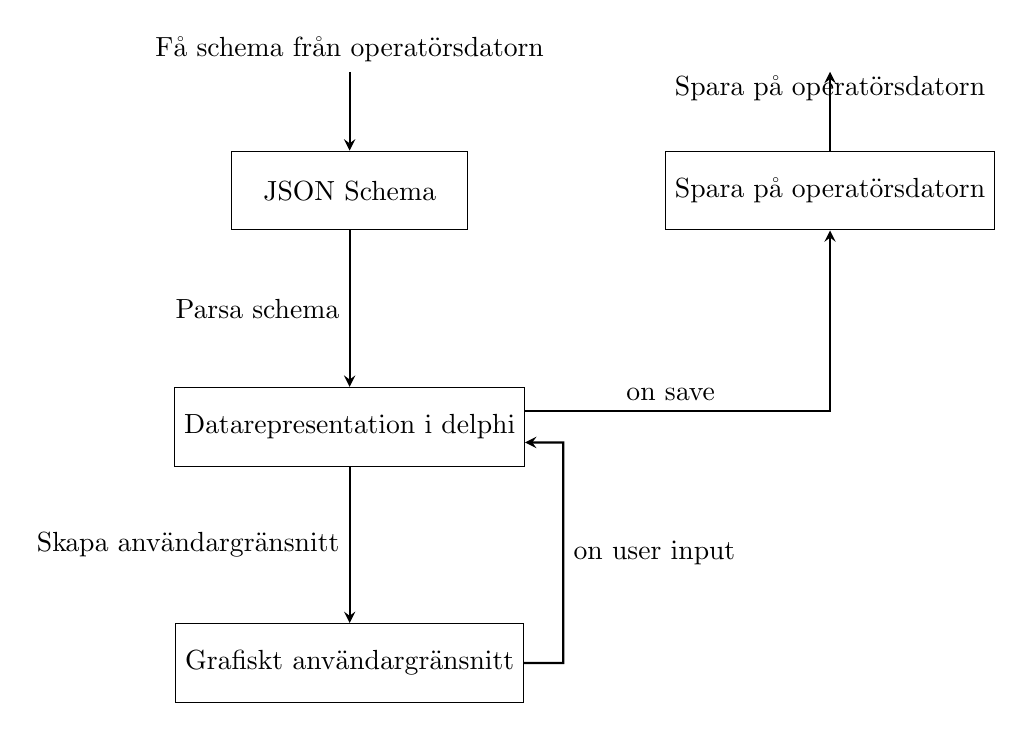
\begin{tikzpicture}
		\node (origin) [defaultnode] {JSON Schema};
		\node (data) [defaultnode, below of=origin, yshift=-2cm] {Datarepresentation i delphi};
		\node (gui) [defaultnode, below of=data, yshift=-2cm] {Grafiskt användargränsnitt};
		\node (save) [defaultnode, right=of origin, xshift=1.5cm] {Spara på operatörsdatorn};
		
		\draw [arrow] (origin) -- node[anchor=east] {Parsa schema} (data);
		\draw [arrow] (data) -- node[anchor=east] {Skapa användargränsnitt} (gui);
		\draw [arrow] (gui.east) -- ++(.5, 0) -- node[anchor=west] {on user input} ++(0, 2.8) -- ([shift={(0, -0.2)}]data.east);
		\draw [arrow] ([shift={(0, 0.2)}]data.east) --  node[anchor=south] {on save} ++ (3.7, 0) -| (save.south);
	
		\draw [arrow] ([shift={(0, 1)}]origin.north) node[anchor=south] {Få schema från operatörsdatorn} -- (origin.north);
		\draw [arrow] (save) -- node[anchor=south] {Spara på operatörsdatorn} ([shift={(0, 1)}]save.north);
	\end{tikzpicture}
\end{figure}

% TODO: Förklara parse

\subsection{Example diagram with TikZ}
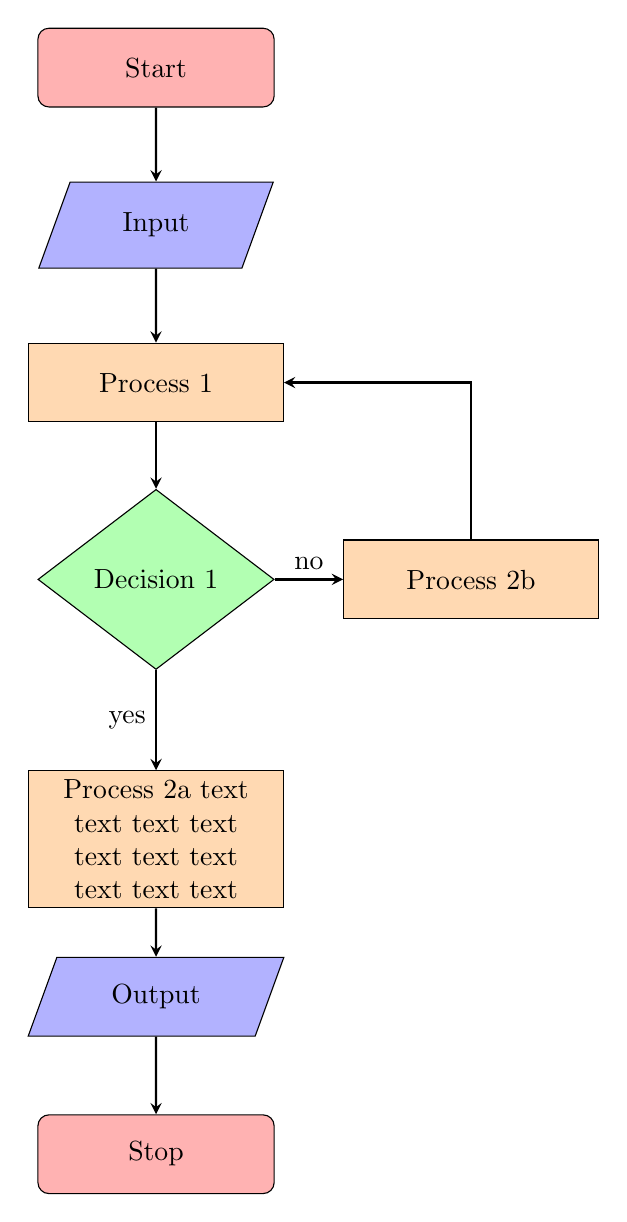
\begin{tikzpicture}[node distance=2cm]
	\node (start) [startstop] {Start};
	\node (in1) [io, below of=start] {Input};
	\node (pro1) [process, below of=in1] {Process 1};
	\node (dec1) [decision, below of=pro1, yshift=-0.5cm] {Decision 1};
	\node (pro2a) [process, below of=dec1, yshift=-1.3cm] {Process 2a text text text text text text text text text text};
	\node (pro2b) [process, right of=dec1, xshift=2cm] {Process 2b};
	\node (out1) [io, below of=pro2a] {Output};
	\node (stop) [startstop, below of=out1] {Stop};
	
	\draw [arrow] (start) -- (in1);
	\draw [arrow] (in1) -- (pro1);
	\draw [arrow] (pro1) -- (dec1);
	\draw [arrow] (dec1) -- node[anchor=east] {yes} (pro2a);
	\draw [arrow] (dec1) -- node[anchor=south] {no} (pro2b);
	\draw [arrow] (pro2b) |- (pro1);
	\draw [arrow] (pro2a) -- (out1);
	\draw [arrow] (out1) -- (stop);
\end{tikzpicture}


\chapter{Resultat}

\section{Vad saknas i JSON Schema}
Hur hanterar man olika valideringsfel?

Föreslå kanske att JSON Schemat som föreslogs i rapport X ska användas.

\section{Hur ska schemat genereras?}

\section{Ett schema för att beskriva schemat}

\section{Datarepresentation i Delphi}
Många språk skiljer på integer och double men det gör varken Javascript, JSON eller JSON Schema


\subsection{JSON Pointer and \$ref}

\section{Användargränsnittet}

\subsection{JSON Editor}
% Vanlig json editor

\subsection{Generaliserat användargränsnitt}
% Nestad form ischhhhhh
	% går ej pga för många inställningar och möjligtvis för djup nestning

\subsection{Användargränsnitt utifrån specifika krav på schemat}
\begin{figure}
	\begin{subfigure}{\textwidth}
		\centering
		\begin{minted}[tabsize=2, frame=lines, fontsize=\small, framesep=2mm]{json}
{
	"$schema": "http://json-schema.org/draft-07/schema",
	"type": "object",
	"properties": {
		"TMimerMainSettings": {
			"title": "Mimer Main Settings",
			"description": "The main settings to set.",
			"type": "object",
			"properties": {
				"MyName": {
					"title": "My Name",
					"description":
						"This is the name that will be shown on a place",
					"type": "string",
					"default": ""
				}
			}
		}
	}
}
		\end{minted}
		\subcaption{Exempel på enkelt JSON Schema}
		\vspace{2em}
	\end{subfigure}
	\begin{subfigure}{\textwidth}
		\centering
		Här ska det finnas en bild med resultatet
		\subcaption{Det resulterande användargränsnittet}
	\end{subfigure}
	\caption{Exempel på enkelt JSON Schema}
\end{figure}

\chapter{Diskussion, slutsats och fortsatt arbete}

\printbibliography[heading=bibintoc] % Print the bibliography (and make it appear in the table of contents)

\appendix

\chapter{API-beskrivning}
\label{appendix:api-beskrivning}

\chapter{Extra Material som Bilaga}

\end{document}
